
\documentclass[acmsmall]{acmart}

%%
%% \BibTeX command to typeset BibTeX logo in the docs
\AtBeginDocument{%
  \providecommand\BibTeX{{%
    \normalfont B\kern-0.5em{\scshape i\kern-0.25em b}\kern-0.8em\TeX}}}


\usepackage{subcaption}
\usepackage{siunitx}

\begin{document}


\title{pyTracer, a raytracer engine made from scratch in Python}

\author{Valentin Taillandier}
\email{taillandier-valentin@g.ecc.u-tokyo.ac.jp}
\affiliation{%
  \institution{The University of Tokyo}
  \streetaddress{7 Chome-3-1 Hongo, Bunkyo City}
  \city{Tokyo}
  \state{Japan}
  \postcode{113-8654}
}

%%
%% By default, the full list of authors will be used in the page
%% headers. Often, this list is too long, and will overlap
%% other information printed in the page headers. This command allows
%% the author to define a more concise list
%% of authors' names for this purpose.
\renewcommand{\shortauthors}{Valentin Taillandier}

%%
%% The abstract is a short summary of the work to be presented in the
%% article.
\begin{abstract}
We made a basic ray-tracer engine in Python from scratch that supports spheres and triangles and can also load meshes in the obj format.
We used the path-tracing scheme to generates rays and simulates Lambertian lighting and Snell-Descartes reflection and refraction (using Fresnel coefficients).
Since ray-tracers involve a lot of geometrical calculations, we had to implement some optimization schemes such as acceleration data-structure or tracing packs of rays with SIMD support.

\end{abstract}


%%
%% Keywords. The author(s) should pick words that accurately describe
%% the work being presented. Separate the keywords with commas.
\keywords{ray-tracing, path-tracing}


%%
%% This command processes the author and affiliation and title
%% information and builds the first part of the formatted document.
\maketitle

\section*{Introduction}
This project is part of a course taken at the University of Tokyo which is an introduction to image synthesis.
A ray-tracer is a kind of 3D engine that traces and simulates light rays to compute colors. 
This involves various scientific fields such as Euclidean geometry (for rays intersections and reflections with objects), photometry (for color computations), and computer sciences (for computational optimization).
Not all reflection rays can be computed and, however, some heuristics exist to set the number of reflections for each ray of light.
Since a lot of rays traced from the light source are lost and do not hit the camera, we use Fermat's backward principle to compute rays from the camera and check if the ray finally hits a light source.
This allows us to trace a fixed amount of rays defined by the resolution of the screen we are projecting the image on.
Some mandatory tasks were defined to frame the project all along with the three different assignments:
\begin{description}
\item[Triangle intersection] We were provided three 3D objects defined as a set of triangles. It was natural to start by implementing triangle intersections. For each vertex of triangles,
a normal vector is provided. From that, it was also mandatory to implement barycentric normal interpolations known as Phong interpolation.
\item[Acceleration data-structure] Ray-tracers involve a lot of geometrical computations. For each pixel of the final picture, the naive way is to try to intersect a ray with each object in the scene.
A simple calculation can show that this is not computationally tractable and we had to implement a data-structure to navigate among the objects with the divide-and-conquer principle.
For personal preferences, we decided to implement BVH with the SAH heuristic.
\item[Statistics] We had to provide statistics such as the number of rays traced per second or the number of object intersection tests for a pixel.

\item[Shadows rays] Simulate shadow when a ray cannot reach the light source.
\item[Shading models] Simulate reflections and refraction using Snell-Descartes laws and Fresnel laws.
\item[HDR image-based lighting] Using light probes to simulate 360\si{\degree} lights sources all around the camera from a real picture.

\item[Depth of field] Simulate depth of field and focalization by simulating a thin lens.
\item[Tone mapping] Implement an algorithm to convert HDR data to RGB pictures.

\item[Path-tracing] Implement a path-tracing algorithm using the Monte-Carlo sampling scheme.
\item[Advanced rendering algorithm] Implement an advanced algorithm. We chose to implement a selective and adaptive path-tracing scheme that is smarter than Monte-Carlo.
\end{description}

This report presents the state of the project, the problems we faced, and provides some results.
The sections are sorted by chronological order to show the evolution of the project over the three assignments.

\section{The project structure}
We adopted the Object-Oriented Programming style which is very convenient for that kind of project. Some classes come naturally:
\subsection*{The engine class}
This class (see fig.~\ref{fig:engine}) takes a central place in our project and links everything together.
\begin{figure}[h]
    \centering
    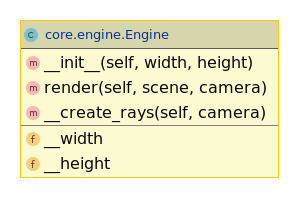
\includegraphics[scale=0.3]{img/engine.pdf}
    \caption{The engine class.}
    \label{fig:engine}
\end{figure}

The \emph{\_\_init\_\_} method is the one that is called when instantiating an object. We provide it the image's width and height in pixels.
The most important method is the \emph{render} that we call to build the picture. This method takes a scene object and a camera object computes the rays issued from the camera and returns it to the scene. For each ray, the scene computes if an object is hit and returns data about the object and the distance from the camera and the object to the engine.
The engine will then use that information to computes colors for each pixel of the picture.
\subsection*{The camera class}
This class (see fig.~\ref{fig:camera}) builds a camera object that will define the origins and directions of the rays.
\begin{figure}[h]
    \centering
    \includegraphics[scale=0.3]{img/camera.pdf}
    \caption{The camera class.}
    \label{fig:camera}
\end{figure}
The most important method here is \emph{\_\_init\_\_} used to build the camera. It takes a position point, two-directional vectors (horizontal and vertical directions), and a number for the \textit{fov}.
The \textit{fov} stands for the horizontal field of view and define the angle in radiant between the rays issued for the most left and right pixels.
\subsection*{The scene and light class}
This scene class (see fig.~\ref{fig:scene}) builds an object that will store the component of the scene we want to render.
It links the engine and all of the 3D objects of the scene.
The light object builds a simple radial isotropic light source, since it is very simple we won't describe it there.
\begin{figure}[h]
    \centering
    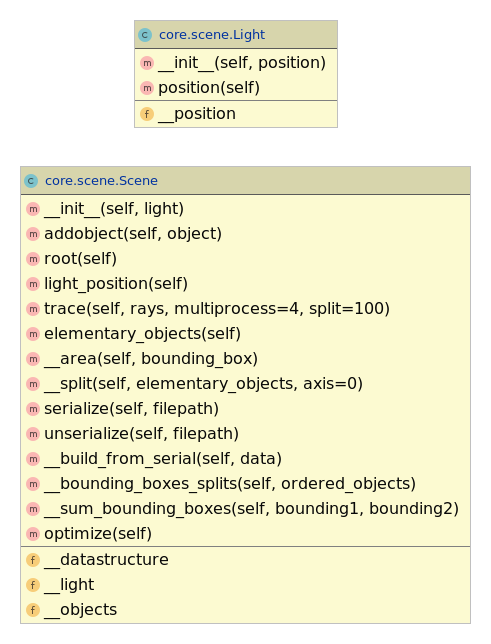
\includegraphics[scale=0.3]{img/scene.pdf}
    \caption{The scene and light class.}
    \label{fig:scene}
\end{figure}
The most important methods of the scene objects are \emph{trace}, \emph{optimize}, \emph{serialize} and \emph{unserialize}.
\emph{trace} gives the rays from the engine to every 3D objects, collects and gathers the intersection data.
\emph{optimize} is called to optimize the data-structure of objects and implement BVH and SAH.
\emph{serialize} and \emph{unserialize} are called to save and load scenes and their data-structures.
Since the \emph{optimize} method can be slow in some cases, we found it very convenient to have a way to save the work done.
The serialized scenes are simple JSON language files that reflect the tree structure of the scene.

\subsection*{The objects classes}
Several classes implement 3D objects such as triangles, spheres, groups and meshes (see fig.~\ref{fig:object}). They all inherit from a global abstract \emph{object} class.
\begin{figure}[h]
    \centering
    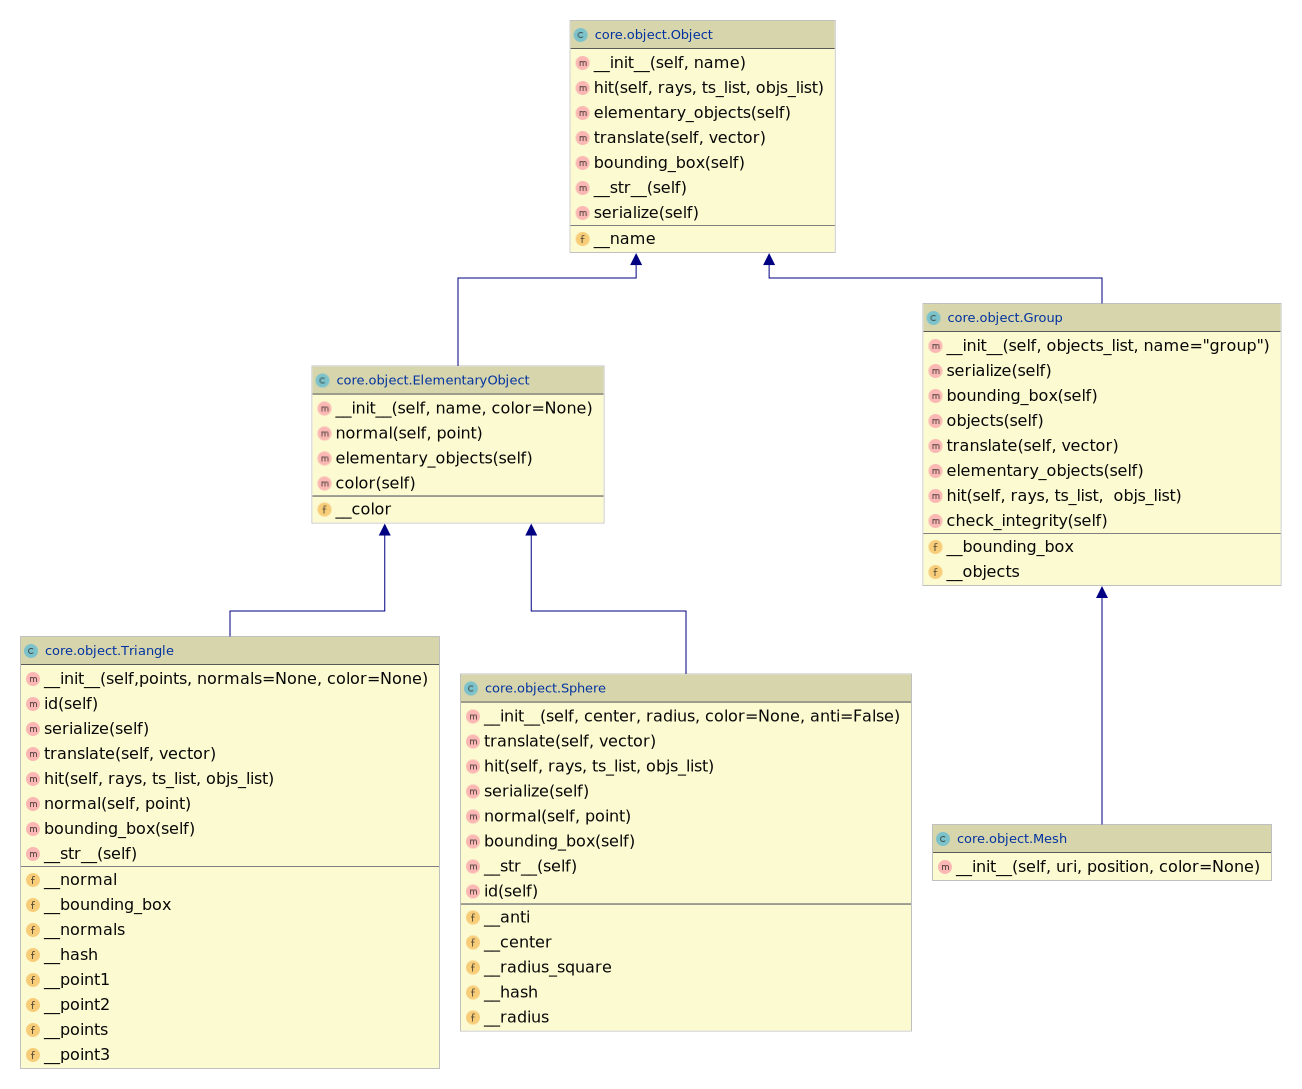
\includegraphics[scale=0.3]{img/object.pdf}
    \caption{The objects classes.}
    \label{fig:object}
\end{figure}

Two classes \emph{Group} and \emph{ElementaryObject} represent respectively the inner nodes and leaves of the tree structure of the scene.
The \textit{Group} class implements the \textit{AABB} test for the data-structure traversal while commentary objects implement their intersection methods and normal computations based on a geometrical formula.
The \emph{Mesh} class is just a special \textit{Group} class that offers a method used to load 3D objects in the .obj format.


\section{Optimization}
\subsection*{The data structure}
We decided to implement the Bounding Volume Hierarchy algorithm known as BVH to recursively split a scene into two sub-scenes.
The Surface Area Heuristic was used to select the best split from every candidate.
Some dynamic programming optimization was made to compute the candidates faster, however, the construction of the data structure is not linear in the number of objects.
Every elementary object implements a bounding box computation method that is called to get the smallest axis-aligned box that is bounding the object.
This smallest box is used by the BVH algorithm to computes the bounding box of the object group resulting in the construction of a candidate.
The resulting data-structures can be serialized and saved to be loaded and reused later.
Figure~\ref{fig:dsteapot} shows an example of a scene rendered with a resolution of $1000\times1000$ pixels and a representation of the number of nodes traversals in the data-structure optimized by BVH.
For each pixel, we computed the number of group nodes traversed and tested elementary objects. The brighter the pixel is, the more intersection computations have been made. This representation naturally shows the
topology of the optimized data-structure. Figure~\ref{fig:dsbunny} shows the same result but for the bunny.

\begin{figure}[h]
    \centering
    
\begin{subfigure}{.5\textwidth}
  \centering
  \includegraphics[width=.9\linewidth]{img/teapot.png}
\end{subfigure}%
\begin{subfigure}{.5\textwidth}
  \centering
  \includegraphics[width=.9\linewidth]{img/tbteapot.png}
\end{subfigure}    
    
    \caption{An image rendered from the teapot 3D objects and a representation of the number of nodes traversals in the corresponding optimized data-structure.}
    \label{fig:dsteapot}
\end{figure}

\begin{figure}[h]
    \centering
    
\begin{subfigure}{.5\textwidth}
  \centering
  \includegraphics[width=.9\linewidth]{img/bunny.png}
\end{subfigure}%
\begin{subfigure}{.5\textwidth}
  \centering
  \includegraphics[width=.9\linewidth]{img/tbbunny.png}
\end{subfigure}    
    
    \caption{An image rendered from the bunny 3D objects and a representation of the number of nodes traversals in the corresponding optimized data-structure.}
    \label{fig:dsbunny}
\end{figure}

\subsection*{Packs of rays and SIMD}
We did a massive \textit{numpy} implementation that allows us to do computations with compiled C code and support of SIMD. In the modern processors, SIMD allows doing computations of 128-bits operands,
which represents four 32-bits operands computations at a time.
For each tested objects, the candidate rays are processed as a single ray.
We observed a substantial improvement in the computation duration.
\subsection*{Multithreading}
We used the \emph{multiprocessing} Python library to distribute work among every CPU's thread. For instance, with a four-core CPU, the image will be divided into 4 and every unit will compute a piece.
We faced a problem with the memory allocation used by this optimization since the scene was copied for each thread. Future work would be to use the BVH data-structure to give the relevant part of the scene to each thread. 

\section{Cosmetic}
\subsection*{Photometry}
For each pixel, we computed the brightness as a sum of the ambient, diffuse and specular brightnesses. This is the so-called Phong's model.
The diffuse and specular brightnesses depend on the normals of the hit objects and the angle of incident and reflected rays.
Computing the reflected rays is done by applying Descartes's law of reflection (the reflected ray is the opposite of the symmetry of the incident ray by the normal of the hit object). 
Figure~\ref{fig:lightteapot} shows the contribution of each nature of luminosities.
 

\begin{figure}[h]
    \centering
    
\begin{subfigure}{.3\textwidth}
  \centering
  \includegraphics[width=.9\linewidth]{img/ambientteapot.png}
\end{subfigure}%
\begin{subfigure}{.3\textwidth}
  \centering
  \includegraphics[width=.9\linewidth]{img/diffuseteapot.png}
\end{subfigure} %
\begin{subfigure}{.3\textwidth}
  \centering
  \includegraphics[width=.9\linewidth]{img/specularteapot.png}
\end{subfigure}    
    
    \caption{From left to right we sequentially add ambient, diffuse and specular lighting.}
    \label{fig:lightteapot}
\end{figure}

\subsubsection*{Phong interpolation}
We implemented barycentric interpolations of normals that gives a smooth aspect to surfaces composed of triangles. We computed normal maps to show improvement.
The Figure~\ref{fig:normalteapot} shows the improvement made on the teapot object. The Figure~\ref{fig:normalsponza} show the same improvement for the Sponza Palace.
\begin{figure}[h]
    \centering
    
\begin{subfigure}{.5\textwidth}
  \centering
  \includegraphics[width=.9\linewidth]{img/nnteapot.png}
\end{subfigure}%
\begin{subfigure}{.5\textwidth}
  \centering
  \includegraphics[width=.9\linewidth]{img/nteapot.png}
\end{subfigure}    
    
    \caption{Normal maps of the teapot with and without Phong interpolation.}
    \label{fig:normalteapot}
\end{figure}

\begin{figure}[h]
    \centering
    
\begin{subfigure}{.5\textwidth}
  \centering
  \includegraphics[width=.9\linewidth]{img/nnsponza.png}
\end{subfigure}%
\begin{subfigure}{.5\textwidth}
  \centering
  \includegraphics[width=.9\linewidth]{img/nsponza.png}
\end{subfigure}    
    
    \caption{Normal maps of the Sponza palace with and without Phong interpolation.}
    \label{fig:normalsponza}
\end{figure}
We planned to implement Phong tessellation, but the intersection test was very difficult to make and we focused on other points.

\section{Benchmark}

Four scenes were provided to make statistics on our implementation. We could not implement the scene with 20 bunnies because our implementation does not support object rotation.
However, we could recreate the three other ones. Figure~\ref{fig:benchmark} shows the recreated scenes. The images were rendered in $512\times512$ (262144 rays in total for each image).
Figure~\ref{fig:benchmarktable} shows the statistics computed.

\begin{figure}[h]
    \centering
    
\begin{subfigure}{.3\textwidth}
  \centering
  \includegraphics[width=.9\linewidth]{img/benchmarkteapot.png}
\end{subfigure}%
\begin{subfigure}{.3\textwidth}
  \centering
  \includegraphics[width=.9\linewidth]{img/benchmarkbunny.png}
\end{subfigure} %
\begin{subfigure}{.3\textwidth}
  \centering
  \includegraphics[width=.9\linewidth]{img/benchmarksponza.png}
\end{subfigure}    
    
    \caption{Three of the benchmark scenes were recreated to be compatible with our implementation.}
    \label{fig:benchmark}
\end{figure}


\begin{figure}
\centering
\small{
\begin{tabular}{c|cccccc}
     & \#Nodes    &  \#Leaves   & \#Ray traversals    & \#Triangle intersections    & Optimization (BVH)    & Rendering   \\ \hline
  Teapot  & 695 &  577 &  5845260 &  1600870 &  0sec &  5sec \\
  Bunny  & 82905 &  69452 &  1469106 &  522947 &  45sec &  26sec \\
  Sponza  & 78039 &  66454 &  44084644 &  7376469 &  43sec &  37sec \\
  
\end{tabular}
}
    \caption{Statistics made from the three rendered scenes.}
    \label{fig:benchmarktable}
\end{figure}


\section{Shadow rays}
To compute color shading for the Lambertian model in the case of punctual light sources, we have to trace rays from the object to the light source and compute the cosine between this ray and the normal of the object.
Until now, we didn't trace the ray to the light source but just compute the direction. The object would look illuminated by the light even if an obstacle is present between the object and the light.
Tracing an actual ray and asserting that it can reach the light source let us compute shadows.
The figure \ref{fig:shadow} shows the same scene with and without shadows. One can remarks that the neck of the teapot has its own shadow on the teapot itself.

\begin{figure}[h]
    \centering
    
\begin{subfigure}{.5\textwidth}
  \centering
  \includegraphics[width=.9\linewidth]{img/withshadow.png}
\end{subfigure}%
\begin{subfigure}{.5\textwidth}
  \centering
  \includegraphics[width=.9\linewidth]{img/withoutshadow.png}
\end{subfigure}    
    
    \caption{The same scene rendered with and without shadows. The light becomes from the right}
    \label{fig:shadow}
\end{figure}

\section{HDR image based lighting}
We implemented the use of HDR image light probes from the website \url{https://www.pauldebevec.com/Probes/}.
We especially used the pfm format of \textit{Grace Cathedral, San Francisco} and \textit{St. Peter's Basilica, Rome}.
The figure \ref{fig:hdrprobes} shows the result of using those hdr images files.
\begin{figure}[h]
    \centering
    
\begin{subfigure}{.5\textwidth}
  \centering
  \includegraphics[width=.9\linewidth]{img/grace.png}
\end{subfigure}%
\begin{subfigure}{.5\textwidth}
  \centering
  \includegraphics[width=.9\linewidth]{img/stpeters.png}
\end{subfigure}    
    
    \caption{The same scene with water spheres using respectively \textit{Grace Cathedral, San Francisco} and \textit{St. Peter's Basilica, Rome}light probes. }
    \label{fig:hdrprobes}
\end{figure}


\section{Shading Models}

\subsection{Specular shading}
We first add specular reflection and refraction to our model thanks to Snell-Descartes laws and Fresnel laws.
We can define in the program the number of bounces we want to compute for each ray from the camera.
Also, we can give a different index to each object as the figure \ref{fig:reflecrefrac} show with different materials (mirrors and water).
Figure \ref{fig:reflec} shows the reflection of a teapot on a sphere.
\begin{figure}[h]
    \centering
    

  \includegraphics[width=.6\linewidth]{img/refracreflec.png}

    
    \caption{Totally reflecting (mirror, eta << 1) teapot and water spheres (eta=1.33).}
    \label{fig:reflecrefrac}
\end{figure}

\begin{figure}[h]
    \centering
    

  \includegraphics[width=.6\linewidth]{img/reflec.png}

    
    \caption{Reflection of a teapot on a sphere.}
    \label{fig:reflec}
\end{figure}

\subsection{Lambertian shading}
In the case of using light probes, any possible directions of light should be taken into account to render the color on the surface of an object.
We then sample random directions of light with a distribution following the Lambertian law which says that the participation of a direction of an incidence ray
of light is proportional to the cosine between it and the normal on the surface of the object.
Images are noisy because not enough samples are taken. Figure \ref{fig:lambertian} shows the effect on a different number of samples.

\begin{figure}[h]
    \centering
    
\begin{subfigure}{.3\textwidth}
  \centering
  \includegraphics[width=.9\linewidth]{img/10.png}
\end{subfigure}%
\begin{subfigure}{.3\textwidth}
  \centering
  \includegraphics[width=.9\linewidth]{img/50.png}
\end{subfigure} %
\begin{subfigure}{.3\textwidth}
  \centering
  \includegraphics[width=.9\linewidth]{img/1000.png}
\end{subfigure}    
    
    
    \caption{The same scene including a teapot with diffuse surface (lambertian) with repectively 10, 50 and 1000 iterations. }
    \label{fig:lambertian}
\end{figure}


\section{Thin lens and depth of field}
We implemented a thin lens model with two parameters: the radius of the lens and the distance of focalization.
To simulate a blur when an object is not at the distance of focalization, we need to sample a ray from the camera to the lens for each coordinate on the disc surface of the lens.
For that, we sample a ray at random uniformly on the surface of the lens.
Figure \ref{fig:lens} shows the effect of using a thin lens to simulate depth of field.

\begin{figure}[h]
    \centering
    
\begin{subfigure}{.5\textwidth}
  \centering
  \includegraphics[width=.9\linewidth]{img/lens1.png}
\end{subfigure}%
\begin{subfigure}{.5\textwidth}
  \centering
  \includegraphics[width=.9\linewidth]{img/lens10.png}
\end{subfigure} 
    
    
    \caption{The same scene with a thin lens and respectively 1 and 10 iterations. }
    \label{fig:lens}
\end{figure}

\section{Tone mapping}
We first tried to implement a naïve tone mapping algorithm:
\[cell := (cell- min)/(max-min) \] 
where $min$ and $max$ are the minimal and maximal values in the HDR image for all RGB canals.
This gave us very dark images with small bright dots.
After investigating on the distributions of the values on the HDR image we decided to correct the previous algorithm with the next formula:
\[ cell := (cell- percentile(5))/(percentile(95)-percentile(5)) \]
where $percentile(x)$ is that $x$\% of the cells have a value under $percentile(x)$.
This gave the results shown on figure \ref{fig:tone}.
The figure \ref{fig:disttone} shows the distribution of values using the naïve or the better tone mapping formula.
We remark that in the first graphic (for the naïve mapping) that almost all cells are near 0 and there are a few cells with value 1.
We also implemented a gamma correction algorithm but we find there is no need to apply it.


\begin{figure}[h]
    \centering
    
\begin{subfigure}{.5\textwidth}
  \centering
  \includegraphics[width=.9\linewidth]{img/withouttone.png}
\end{subfigure}%
\begin{subfigure}{.5\textwidth}
  \centering
  \includegraphics[width=.9\linewidth]{img/withtone.png}
\end{subfigure} 
    
    \caption{The same scene with the naïve tone mapping and the better one. }
    \label{fig:tone}
\end{figure}

\begin{figure}[h]
    \centering
    
\begin{subfigure}{.5\textwidth}
  \centering
  \includegraphics[width=.9\linewidth]{img/withouttone.pdf}
\end{subfigure}%
\begin{subfigure}{.5\textwidth}
  \centering
  \includegraphics[width=.9\linewidth]{img/withtone.pdf}
\end{subfigure} 
    
    \caption{The values distribution with the naïve tone mapping and the better one.}
    \label{fig:disttone}
\end{figure}


\section{Path-Tracing}
We implemented path-tracing using Monte-Carlo to randomly sample a ray for a pixel and randomly choose the behavior when a ray hit a surface.
For instance, on a dielectric surface, a ray can be both reflected and refracted. The energy of the incident ray is then spitted in two according to the Fresnel coefficients.
Those coefficients are positive and sum up to 1 so that they can be used as the probability that a photon is reflected or refracted. We use this behavior in our path-tracing algorithm.
For a Lambertian surface, a ray is randomly reflected in a cone of reflection. The angle between the incident ray and the reflected one is a random variable and can be simulated with the Monte-Carlo method.

Path-Tracing consists to set maximum depths for ray bounces (including reflection and refraction). When tracing a ray, each bounce results in only one sub-ray which makes the algorithm linear and not exponential to the number of maximum depths.
Since the algorithm is randomized, we need to repeat the computation many times to compute an average from the results of every ray belonging to a pixel.
Because we can throw many rays for only one pixel on the picture, we are allowed to throw random directions inside the pixel area. To be more precise, a pixel can be seen as a point but also as a surface that receives light from many ray directions. We use randomness again to generates directions. This results in solving the problem of spatial aliasing. The image seems more smooth and accurate.

\section{Adaptive Path-Tracing}
Some parts of a rendered picture involve a lot of randomnesses and then noise. Especially for diffuse material since a bouncing ray can be reflected in a lot of various directions.
The picture in figure \ref{fig:noise} shows a path-traced scene with 20 samples. That means that every pixel is computed as an average of 20 computations.
This picture shows a lot of noise, especially on diffuse materials. A naive solution would be to increase the number of samples for every pixels.
This solution is time consuming and not very smart since some pixels do not need a lot of computation.
\begin{figure}[h]
    \centering
    
  \includegraphics[width=.6\linewidth]{img/noise.png}
    
    \caption{Path-traced scene including a diffuse material teapot (on the right) with a lot of noise.}
    \label{fig:noise}
\end{figure}

We then came up with another solution which is an adaptive path-tracing.
The idea is to iteratively compute samples for pixels and stop when the average of computations has converged.
More formally, for every pixel to render we define $a^{x,y}_n$, the value computed at iteration $n$ for pixel $(x,y)$. We then can define the partial average $m^{x,y}_n$:
\[m^{x,y}_n = \frac{1}{n} \sum^{n}_{i=1}a^{x,y}_i\]
We can study the difference between the partial average at two different iterations:
\begin{align}
| m^{x,y}_{n+1} -m^{x,y}_{n} | &=  \frac{1}{n+1}|a^{x,y}_{n+1} -  m^{x,y}_{n}|\\
\end{align}
We define a threshold $\epsilon$ which helps us to know when to stop the computation. If the absolute value of differences between the average of two iterations is lower than epsilon, we stop the computation.
For more stability we can force several iteration before using the $\epsilon$ criterion.

For a maximum of one thousand of computations per pixel, we obtained the image on figure \ref{fig:adaptive}.

\begin{figure}[h]
    \centering
    
\begin{subfigure}{.5\textwidth}
  \centering
  \includegraphics[width=.9\linewidth]{img/denoised.png}
\end{subfigure}%
\begin{subfigure}{.5\textwidth}
  \centering
  \includegraphics[width=.9\linewidth]{img/compute.png}
\end{subfigure} 
    
    \caption{Experiments with the adaptive method for a maximum of one thousand computations per pixels. The figure on the right represents the number of computations per pixel (dark-blue is 1 and yellow is 1000).}
    \label{fig:adaptive}
\end{figure}
We can observe that this scheme leads to more computations for pixels having more randomness in their samples. However, we observe the most noised areas do not perfectly fit with this.
There are two kinds of noises. The first one is temporal noise, which is the noise between the samples of different iterations for the same pixel. The second one is spatial noise, between the samples of two adjacent pixels.
Our solution doesn't solve spatial noise but could be adapted to another scheme.



\end{document}
\endinput
%%
%% End of file `sample-acmsmall.tex'.

